\documentclass[main.tex]{subfiles}

\begin{document}

%\custompart{Quantifier l'\hetero d'une tumeur à partir d'une image}{Comment ? Par quel biais? Exploration de différents critères.}{Dans cette partie, on propose d'examiner en détail le caractère \heterogene de nos images - les images médicales ainsi que les images produites numériquement avec le modèle EDP. Dans un premier temps, nous présenterons la construction d'histogrammes des niveaux de gris contenus dans l'image. Dans un second temps, nous décrirons ces histogrammes par un mélange de gaussienne. Enfin ce mélange gaussien sera utilisé pour calculer différents critères qui seront comparés. }

%\chapter{Construction des histogrammes de niveaux de gris}
%\chapter{Fit des histogrammes}
%\todo[noline]{On peut employer le mot "fit" ?}


\chapter{Critère quantifiant l'\hetero.}
%\lettrine[lines=2, lhang=0.33, loversize=0.25]{$\mathscr{D}$}{ans} 
\lettrine[lines=2, lhang=0.33, loversize=0.25]{D}{ans} ce chapitre, nous allons construire un critère permettant permettant de quantifier l'\hetero d'une tumeur.
A chaque image, on construira l'histogramme des niveaux de gris associés aux tumeurs. 
Dans un premier temps, les images cliniques seront considérées. Les histogrammes associés à ces scanners (qu'on appelera par abus de langage \og histogramme clinique \fg) seront ensuite étudiés. Plusieurs quantités seront examinées afin de construire un quantificateur de l'\hetero.
Dans un second temps, nous appliquerons le même traitement aux images produites par la simulation numérique du modèle EDP présenté précédemment. Les histogrammes des images produites numériquement (qu'on appelera aussi par abus de langage \og histogramme numérique \fg) seront présentés et comparés à ceux cliniques. De même, le quantificateur de l'\hetero que l'on a construit, sera appliqué aux histogrammes numériques et nous pourrons ainsi voir à quel point le modèle EDP est capable de reproduire les aspects homogènes et \heterogenes des tumeurs que l'on considère.
\section{Construction des histogrammes de niveaux de gris.}
Dans cette section, il s'agit, à partir d'une image donnée en niveaux de gris et d'un contour donné, de reconstruire l'histogramme des niveaux de gris des pixels présents à l'intérieur du contour. Une telle zone est communément appelée ROI (de l'anglais: Region Of Interest). Dans la suite, pour une image donnée, on notera $p(\vecx)$ la valeur du pixel (comprise entre 0 et 255) situé en position $\vecx$. Ainsi les données de l'histogramme sont représenté par la liste (ensemble avec valeur multiples autorisées)~:
\begin{equation}
\label{eq:def_data_histo}
X:=\{ \ p(\vecx) \  | \  \vecx \in \textrm{\small ROI} \ \},
\end{equation}
et l'histogramme lui-même, que l'on normalise, est donné par la fonction~:
\begin{equation}
\label{eq:def_histo}
H(x) = \dfrac{ \# X_x  }{ \# X }, \qquad \forall x \in \{ 0,1,2,\ldots,255 \}
\end{equation}
où $x$ désigne un niveau de gris et $X_x$ désigne la partition de la liste $X$ qui ne contient que les éléments $x$.

\subsection{Histogrammes cliniques}
\todo[noline]{Description du processus médical pour les scanners: ajout ici ?}
Les données dont nous disposons sont celles produites par le scanner. Beaucoup plus riche qu'une image, ces données au format DICOM, nécéssitent l'utilisation d'un outil adapté pour les visualiser. OsiriX est ainsi utilisé pour:
\begin{itemize}
\item Choisir une coupe pertinente sur chaque scanner et l'exporter (également au format DICOM) de sorte à avoir ensuite des données 2D à traiter.
\item Contourer manuellement la métastase. OsiriX dispose d'un outil crayon adapté à ce type de contourage. Ce contourage définit une ROI, que l'on peut également exporter (au format .xml)
\end{itemize}
A partir de ces 2 fichiers, un code C++, s'appuyant sur la librairie ITK qui traite entre autre le format DICOM, permet de :
\begin{itemize}
\item Construire l'histogramme des niveaux de gris en parcourant  l'ensemble des pixels du scanner contenus uniquement dans la ROI. 
A titre indicatif, l'ensemble des histogrammes cliniques de \Nber et de \Chen sont présentés Figure~\ref{fig:histo_dcm_Nber} et~\ref{fig:histo_dcm_Chen}. Nous les commenterons plus tard.
\todo[noline]{Commenter les histogrammes}
\item Produire des images sur lesquelles le contour est visible. L'ensemble des contourages effectués pour \Nber et pour \Chen sont présentés respectivement Figure~\ref{fig:contourageNber} et~\ref{fig:contourageChen}.
\todo[noline]{Commenter les contourages?}
\end{itemize}


Remarquons que, comme montré sur la figure~\ref{fig:contourage_sain}, le logiciel OsiriX, permet de visualiser directement l'histogramme des niveaux de gris d'une ROI. Cependant, il n'y a aucune possibilité d'exporter ces histogrammes... De plus on souhaite appliquer autant que possible, un traitement similaire aux images cliniques et aux images numériques, images numériques qui ne peuvent être traiter avec OsiriX. Le développement d'un code pour réaliser ceci était donc nécessaire.


\subsection{Histogrammes numériques}
Pour les histogrammes numériques, seule une image est reconstruite par la simulation. Le contour quant à lui va être définit à partir des fichiers de sorties des simulations qui stockent la densité des différentes populations en chaque maille de notre modèle EDP. En utilisant la reconstruction en niveau de gris détaillée au chapitre précédent, on peut fournir une image en niveaux de gris à partir de ces valeurs. En ce qui concerne le contour, il sera définit par seuillage sur le tissu sain~: si la proportion de tissu sain est inférieur à un pourcentage donné, alors on considèrera que l'on est à l'intérieur de la tumeur, sinon on est à l'extérieure. Nous avons donc également dans cas, une image en niveaux de gris et une ROI. Le code C++ pour la partie clinique peut être réutilisé et produira ainsi les histogrammes numériques.

\subsection{Traitements appliqués aux histogrammes~: fit par un mélange bi-gaussien}

\newlength{\largeurfignber}
\setlength{\largeurfignber}{0.19\textwidth}
%\begin{figure}
%\centering
%\subfloat[Jour 0]{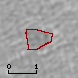
\includegraphics[width=\largeurfignber]{dcm_img/Nber_2008_05_20_scan_contour.png}}\ 
%\subfloat[Jour 119]{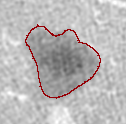
\includegraphics[width=\largeurfignber]{dcm_img/Nber_2008_09_16_scan_contour.png}}\ 
%\subfloat[Jour 209]{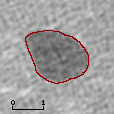
\includegraphics[width=\largeurfignber]{dcm_img/Nber_2008_12_15_scan_contour.png}}\ 
%\subfloat[Jour 275]{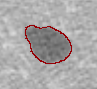
\includegraphics[width=\largeurfignber]{dcm_img/Nber_2009_02_19_scan_contour.png}}\ 
%\subfloat[Jour 331]{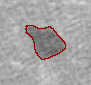
\includegraphics[width=\largeurfignber]{dcm_img/Nber_2009_04_16_scan_contour.png}}\ 
%\subfloat[Jour 406]{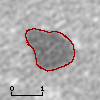
\includegraphics[width=\largeurfignber]{dcm_img/Nber_2009_06_30__slice-244_85_scan_contour.png}}\ 
%\subfloat[Jour 493]{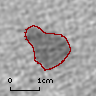
\includegraphics[width=\largeurfignber]{dcm_img/Nber_2009_09_25_scan_contour.png}}\ 
%\subfloat[Jour 535]{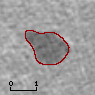
\includegraphics[width=\largeurfignber]{dcm_img/Nber_2009_11_06_scan_contour.png}}\ 
%\subfloat[Jour 611]{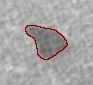
\includegraphics[width=\largeurfignber]{dcm_img/Nber_2010_01_21_scan_contour.png}}\ 
%\subfloat[Jour 688]{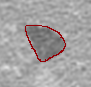
\includegraphics[width=\largeurfignber]{dcm_img/Nber_2010_04_08_scan_contour.png}}\ 
%\subfloat[Jour 776]{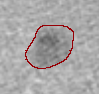
\includegraphics[width=\largeurfignber]{dcm_img/Nber_2010_07_05__slice-263_20_scan_contour.png}}\ 
%\subfloat[Jour 867]{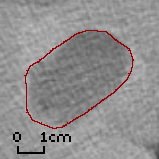
\includegraphics[width=\largeurfignber]{dcm_img/Nber_2010_10_04__slice-239_40_scan_contour.png}}\ 
%\subfloat[Jour 888]{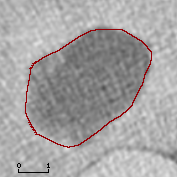
\includegraphics[width=\largeurfignber]{dcm_img/Nber_2010_10_25__slice-246_60_scan_contour.png}}\ 
%\subfloat[Jour 927]{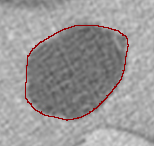
\includegraphics[width=\largeurfignber]{dcm_img/Nber_2010_12_03_scan_contour.png}}\ 
%\subfloat[Jour 962]{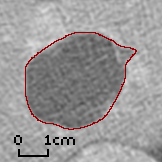
\includegraphics[width=\largeurfignber]{dcm_img/Nber_2011_01_07__slice-221_20_scan_contour.png}}\ 
%\subfloat[Jour 990]{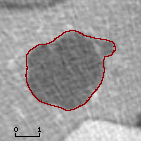
\includegraphics[width=\largeurfignber]{dcm_img/Nber_2011_02_04_scan_contour.png}}\ 
%\subfloat[Jour 1053]{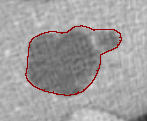
\includegraphics[width=\largeurfignber]{dcm_img/Nber_2011_04_08_scan_contour.png}}\ 
%\subfloat[Jour 1116]{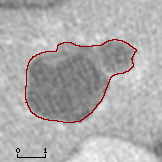
\includegraphics[width=\largeurfignber]{dcm_img/Nber_2011_06_10_scan_contour.png}}\ 
%\subfloat[Jour 1179]{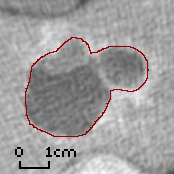
\includegraphics[width=\largeurfignber]{dcm_img/Nber_2011_08_12_scan_contour.png}}
%\caption{\label{fig:contourageNber} Contourage manuel de la tumeur de \Nber. }
%\end{figure}

\begin{figure}
\setlength{\tabcolsep}{1mm} %%% padding horizontal
\begin{tabular}{ccccc}
\subfloat[Jour 0]{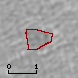
\includegraphics[width=\largeurfignber]{dcm_img/Nber_2008_05_20_scan_contour.png}}&
\subfloat[Jour 119]{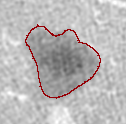
\includegraphics[width=\largeurfignber]{dcm_img/Nber_2008_09_16_scan_contour.png}}&
\subfloat[Jour 209]{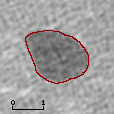
\includegraphics[width=\largeurfignber]{dcm_img/Nber_2008_12_15_scan_contour.png}}&
\multicolumn{2}{c}{%
\multirow{2}{*}[15mm]{
\captionsetup[subfigure]{labelformat=empty}
\vspace{-3cm}
\subfloat[Position des points]{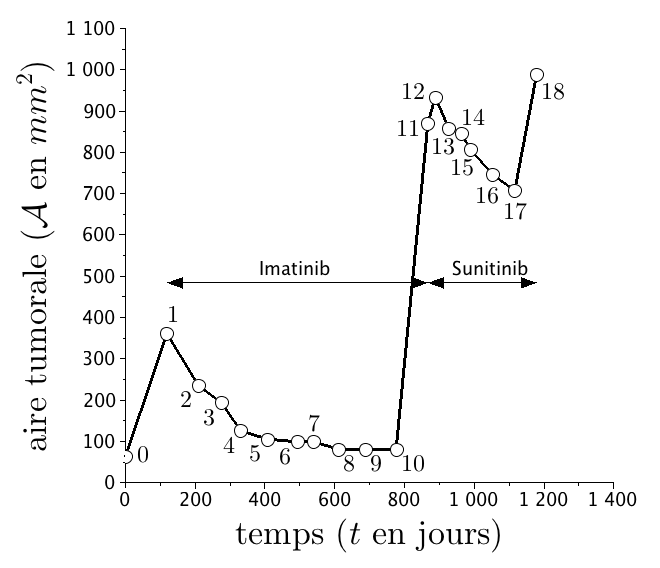
\includegraphics[width=2\largeurfignber]{evo_tps/henbert_listing_point.png}}
\captionsetup[subfigure]{labelformat=parens}
\addtocounter{subfigure}{-1}
}}\\
\subfloat[Jour 275]{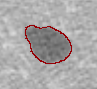
\includegraphics[width=\largeurfignber]{dcm_img/Nber_2009_02_19_scan_contour.png}}&
\subfloat[Jour 331]{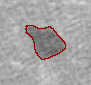
\includegraphics[width=\largeurfignber]{dcm_img/Nber_2009_04_16_scan_contour.png}}&
\subfloat[Jour 406]{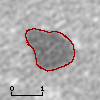
\includegraphics[width=\largeurfignber]{dcm_img/Nber_2009_06_30__slice-244_85_scan_contour.png}}&
\multicolumn{2}{c}{}\\
\subfloat[Jour 493]{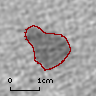
\includegraphics[width=\largeurfignber]{dcm_img/Nber_2009_09_25_scan_contour.png}}&
\subfloat[Jour 535]{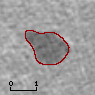
\includegraphics[width=\largeurfignber]{dcm_img/Nber_2009_11_06_scan_contour.png}}&
\subfloat[Jour 611]{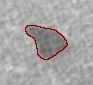
\includegraphics[width=\largeurfignber]{dcm_img/Nber_2010_01_21_scan_contour.png}}&
\subfloat[Jour 688]{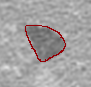
\includegraphics[width=\largeurfignber]{dcm_img/Nber_2010_04_08_scan_contour.png}}&
\subfloat[Jour 776]{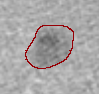
\includegraphics[width=\largeurfignber]{dcm_img/Nber_2010_07_05__slice-263_20_scan_contour.png}}\\
\subfloat[Jour 867]{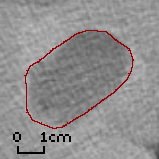
\includegraphics[width=\largeurfignber]{dcm_img/Nber_2010_10_04__slice-239_40_scan_contour.png}}&
\subfloat[Jour 888]{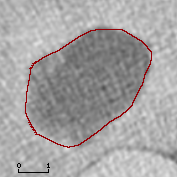
\includegraphics[width=\largeurfignber]{dcm_img/Nber_2010_10_25__slice-246_60_scan_contour.png}}&
\subfloat[Jour 927]{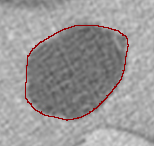
\includegraphics[width=\largeurfignber]{dcm_img/Nber_2010_12_03_scan_contour.png}}&
\subfloat[Jour 962]{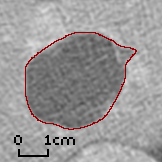
\includegraphics[width=\largeurfignber]{dcm_img/Nber_2011_01_07__slice-221_20_scan_contour.png}}&
\subfloat[Jour 990]{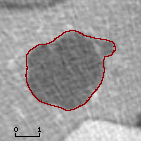
\includegraphics[width=\largeurfignber]{dcm_img/Nber_2011_02_04_scan_contour.png}}\\
&\subfloat[Jour 1053]{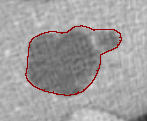
\includegraphics[width=\largeurfignber]{dcm_img/Nber_2011_04_08_scan_contour.png}}&
\subfloat[Jour 1116]{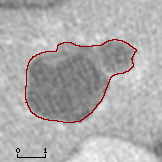
\includegraphics[width=\largeurfignber]{dcm_img/Nber_2011_06_10_scan_contour.png}}&
\subfloat[Jour 1179]{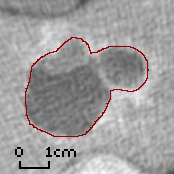
\includegraphics[width=\largeurfignber]{dcm_img/Nber_2011_08_12_scan_contour.png}}
\end{tabular}
\caption{\label{fig:contourageNber} Contourage manuel de la tumeur de \Nber. }
\todo[inline]{Indicateur pour presenter l'echelle sur chaque scan ?}
\end{figure}

%\begin{figure}
%\begin{tabular}{ccccc}
%\subfloat[Jour 0]{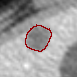
\includegraphics[width=\largeurfignber]{dcm_img/Chen_2007_05_23_scan_contour.png}}&
%\subfloat[Jour 93]{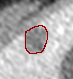
\includegraphics[width=\largeurfignber]{dcm_img/Chen_2007_08_24_scan_contour.png}}&
%\subfloat[Jour 182]{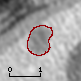
\includegraphics[width=\largeurfignber]{dcm_img/Chen_2007_11_21_scan_contour.png}}\\
%\subfloat[Jour 279]{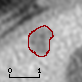
\includegraphics[width=\largeurfignber]{dcm_img/Chen_2008_02_26_scan_contour.png}}&
%\subfloat[Jour 331]{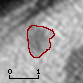
\includegraphics[width=\largeurfignber]{dcm_img/Chen_2008_04_18_scan_contour.png}}&
%\subfloat[Jour 429]{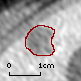
\includegraphics[width=\largeurfignber]{dcm_img/Chen_2008_07_25_scan_contour.png}}&
%\captionsetup[subfigure]{labelformat=empty}
%\subfloat[Position des points]{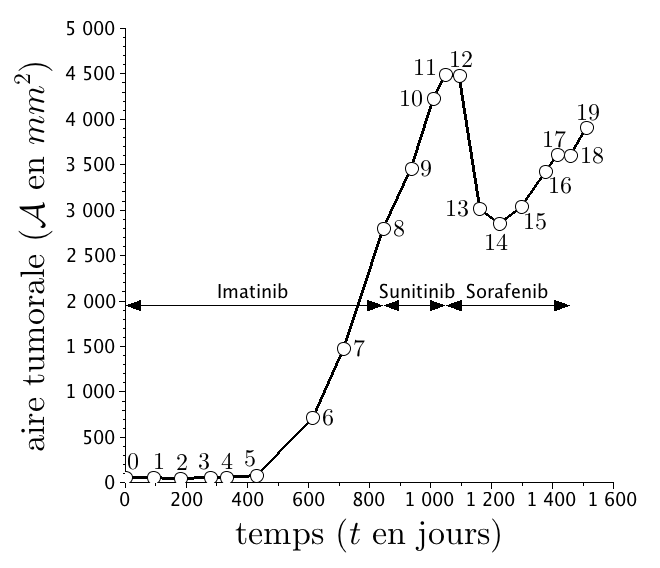
\includegraphics[width=2\largeurfignber]{evo_tps/chen_listing_point.png}}\\
%\captionsetup[subfigure]{labelformat=parens}
%\addtocounter{subfigure}{-1}
%\subfloat[Jour 614]{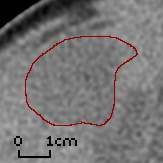
\includegraphics[width=\largeurfignber]{dcm_img/Chen_2009_01_26_scan_contour.png}}&
%\subfloat[Jour 715]{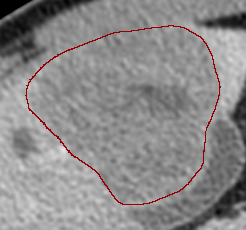
\includegraphics[width=\largeurfignber]{dcm_img/Chen_2009_05_07_scan_contour.png}}&
%\subfloat[Jour 845]{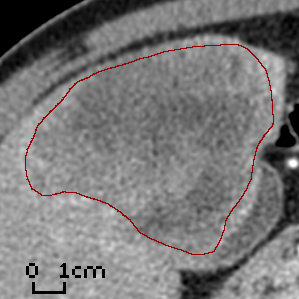
\includegraphics[width=\largeurfignber]{dcm_img/Chen_2009_09_14_scan_contour.png}}&
%\subfloat[Jour 936]{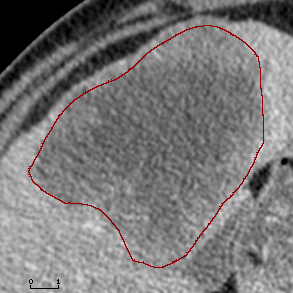
\includegraphics[width=\largeurfignber]{dcm_img/Chen_2009_12_14_scan_contour.png}}&
%\subfloat[Jour 1009]{\includegraphics[width=\largeurfignber]{dcm_img/Chen_2010_02_25_scan_contour.png}}\\
%\subfloat[Jour 1049]{\includegraphics[width=\largeurfignber]{dcm_img/Chen_2010_04_06_scan_contour.png}}&
%\subfloat[Jour 1093]{\includegraphics[width=\largeurfignber]{dcm_img/Chen_2010_05_20_scan_contour.png}}&
%\subfloat[Jour 1161]{\includegraphics[width=\largeurfignber]{dcm_img/Chen_2010_07_27_scan_contour.png}}&
%\subfloat[Jour 1224]{\includegraphics[width=\largeurfignber]{dcm_img/Chen_2010_09_28_scan_contour.png}}&
%\subfloat[Jour 1296]{\includegraphics[width=\largeurfignber]{dcm_img/Chen_2010_12_09_scan_contour.png}}\\
%\subfloat[Jour 1377]{\includegraphics[width=\largeurfignber]{dcm_img/Chen_2011_02_28_scan_contour.png}}& 
%\subfloat[Jour 1415]{\includegraphics[width=\largeurfignber]{dcm_img/Chen_2011_04_07_scan_contour.png}}&
%\subfloat[Jour 1458]{\includegraphics[width=\largeurfignber]{dcm_img/Chen_2011_05_20_scan_contour.png}}& 
%\subfloat[Jour 1510]{\includegraphics[width=\largeurfignber]{dcm_img/Chen_2011_07_11_scan_contour.png}}
%\end{tabular}
%\caption{\label{fig:contourageChen} Contourage manuel de la tumeur de \Chen. }
%\end{figure}

\begin{figure}
\setlength{\tabcolsep}{1mm} %%% padding horizontal
\begin{tabular}{ccccc}
%%% \renewcommand{\arraystretch}{3} %%%% padding vertical (ne semble pas fonctionner
\subfloat[Jour 0]{\includegraphics[width=\largeurfignber]{dcm_img/Chen_2007_05_23_scan_contour.png}}&
\subfloat[Jour 93]{\includegraphics[width=\largeurfignber]{dcm_img/Chen_2007_08_24_scan_contour.png}}&
\subfloat[Jour 182]{\includegraphics[width=\largeurfignber]{dcm_img/Chen_2007_11_21_scan_contour.png}}
&\multicolumn{2}{c}{%
\multirow{2}{*}[15mm]{
\captionsetup[subfigure]{labelformat=empty}
\vspace{-3cm}
\subfloat[Position des points]{\includegraphics[width=2\largeurfignber]{evo_tps/chen_listing_point.png}}
\captionsetup[subfigure]{labelformat=parens}
\addtocounter{subfigure}{-1}
}}\\
\subfloat[Jour 279]{\includegraphics[width=\largeurfignber]{dcm_img/Chen_2008_02_26_scan_contour.png}}&
\subfloat[Jour 331]{\includegraphics[width=\largeurfignber]{dcm_img/Chen_2008_04_18_scan_contour.png}}&
\subfloat[Jour 429]{\includegraphics[width=\largeurfignber]{dcm_img/Chen_2008_07_25_scan_contour.png}}&
\multicolumn{2}{c}{}\\
\subfloat[Jour 614]{\includegraphics[width=\largeurfignber]{dcm_img/Chen_2009_01_26_scan_contour.png}}&
\subfloat[Jour 715]{\includegraphics[width=\largeurfignber]{dcm_img/Chen_2009_05_07_scan_contour.png}}&
\subfloat[Jour 845]{\includegraphics[width=\largeurfignber]{dcm_img/Chen_2009_09_14_scan_contour.png}}&
\subfloat[Jour 936]{\includegraphics[width=\largeurfignber]{dcm_img/Chen_2009_12_14_scan_contour.png}}&
\subfloat[Jour 1009]{\includegraphics[width=\largeurfignber]{dcm_img/Chen_2010_02_25_scan_contour.png}}\\
\subfloat[Jour 1049]{\includegraphics[width=\largeurfignber]{dcm_img/Chen_2010_04_06_scan_contour.png}}&
\subfloat[Jour 1093]{\includegraphics[width=\largeurfignber]{dcm_img/Chen_2010_05_20_scan_contour.png}}&
\subfloat[Jour 1161]{\includegraphics[width=\largeurfignber]{dcm_img/Chen_2010_07_27_scan_contour.png}}&
\subfloat[Jour 1224]{\includegraphics[width=\largeurfignber]{dcm_img/Chen_2010_09_28_scan_contour.png}}&
\subfloat[Jour 1296]{\includegraphics[width=\largeurfignber]{dcm_img/Chen_2010_12_09_scan_contour.png}}
\end{tabular}\\
\begin{tabular}{p{.5\largeurfignber}cccc}
& \subfloat[Jour 1377]{\includegraphics[width=\largeurfignber]{dcm_img/Chen_2011_02_28_scan_contour.png}}& 
\subfloat[Jour 1415]{\includegraphics[width=\largeurfignber]{dcm_img/Chen_2011_04_07_scan_contour.png}}&
\subfloat[Jour 1458]{\includegraphics[width=\largeurfignber]{dcm_img/Chen_2011_05_20_scan_contour.png}}& 
\subfloat[Jour 1510]{\includegraphics[width=\largeurfignber]{dcm_img/Chen_2011_07_11_scan_contour.png}}
\end{tabular}
\caption{\label{fig:contourageChen} Contourage manuel de la tumeur de \Chen. }
\end{figure}


\begin{figure}
\centering
\subfloat[Jour 0]{\includegraphics[width=\largeurfignber]{histo_dcm/Nber_2008_05_20_histo.png}}\ 
\subfloat[Jour 119]{\includegraphics[width=\largeurfignber]{histo_dcm/Nber_2008_09_16_histo.png}}\ 
\subfloat[Jour 209]{\includegraphics[width=\largeurfignber]{histo_dcm/Nber_2008_12_15_histo.png}}\ 
\subfloat[Jour 275]{\includegraphics[width=\largeurfignber]{histo_dcm/Nber_2009_02_19_histo.png}}\ 
\subfloat[Jour 331]{\includegraphics[width=\largeurfignber]{histo_dcm/Nber_2009_04_16_histo.png}}\ 
\subfloat[Jour 406]{\includegraphics[width=\largeurfignber]{histo_dcm/Nber_2009_06_30__slice-244_85_histo.png}}\ 
\subfloat[Jour 493]{\includegraphics[width=\largeurfignber]{histo_dcm/Nber_2009_09_25_histo.png}}\ 
\subfloat[Jour 535]{\includegraphics[width=\largeurfignber]{histo_dcm/Nber_2009_11_06_histo.png}}\ 
\subfloat[Jour 611]{\includegraphics[width=\largeurfignber]{histo_dcm/Nber_2010_01_21_histo.png}}\ 
\subfloat[Jour 688]{\includegraphics[width=\largeurfignber]{histo_dcm/Nber_2010_04_08_histo.png}}\ 
\subfloat[Jour 776]{\includegraphics[width=\largeurfignber]{histo_dcm/Nber_2010_07_05__slice-263_20_histo.png}}\ 
\subfloat[Jour 867]{\includegraphics[width=\largeurfignber]{histo_dcm/Nber_2010_10_04__slice-239_40_histo.png}}\ 
\subfloat[Jour 888]{\includegraphics[width=\largeurfignber]{histo_dcm/Nber_2010_10_25__slice-246_60_histo.png}}\ 
\subfloat[Jour 927]{\includegraphics[width=\largeurfignber]{histo_dcm/Nber_2010_12_03_histo.png}}\ 
\subfloat[Jour 962]{\includegraphics[width=\largeurfignber]{histo_dcm/Nber_2011_01_07__slice-221_20_histo.png}}\ 
\subfloat[Jour 990]{\includegraphics[width=\largeurfignber]{histo_dcm/Nber_2011_02_04_histo.png}}\ 
\subfloat[Jour 1053]{\includegraphics[width=\largeurfignber]{histo_dcm/Nber_2011_04_08_histo.png}}\ 
\subfloat[Jour 1116]{\includegraphics[width=\largeurfignber]{histo_dcm/Nber_2011_06_10_histo.png}}\ 
\subfloat[Jour 1179]{\includegraphics[width=\largeurfignber]{histo_dcm/Nber_2011_08_12_histo.png}}
\caption{\label{fig:histo_dcm_Nber} Histogramme clinique de la tumeur de \Nber. }
\end{figure}

\begin{figure}
\centering
\subfloat[Jour 0]{\includegraphics[width=\largeurfignber]{histo_dcm/Chen_2007_05_23_histo.png}}\ 
\subfloat[Jour 93]{\includegraphics[width=\largeurfignber]{histo_dcm/Chen_2007_08_24_histo.png}}\ 
\subfloat[Jour 182]{\includegraphics[width=\largeurfignber]{histo_dcm/Chen_2007_11_21_histo.png}}\ 
\subfloat[Jour 279]{\includegraphics[width=\largeurfignber]{histo_dcm/Chen_2008_02_26_histo.png}}\ 
\subfloat[Jour 331]{\includegraphics[width=\largeurfignber]{histo_dcm/Chen_2008_04_18_histo.png}}\ 
\subfloat[Jour 429]{\includegraphics[width=\largeurfignber]{histo_dcm/Chen_2008_07_25_histo.png}}\ 
\subfloat[Jour 614]{\includegraphics[width=\largeurfignber]{histo_dcm/Chen_2009_01_26_histo.png}}\ 
\subfloat[Jour 715]{\includegraphics[width=\largeurfignber]{histo_dcm/Chen_2009_05_07_histo.png}}\ 
\subfloat[Jour 845]{\includegraphics[width=\largeurfignber]{histo_dcm/Chen_2009_09_14_histo.png}}\ 
\subfloat[Jour 936]{\includegraphics[width=\largeurfignber]{histo_dcm/Chen_2009_12_14_histo.png}}\ 
\subfloat[Jour 1009]{\includegraphics[width=\largeurfignber]{histo_dcm/Chen_2010_02_25_histo.png}}\ 
\subfloat[Jour 1049]{\includegraphics[width=\largeurfignber]{histo_dcm/Chen_2010_04_06_histo.png}}\ 
\subfloat[Jour 1093]{\includegraphics[width=\largeurfignber]{histo_dcm/Chen_2010_05_20_histo.png}}\ 
\subfloat[Jour 1161]{\includegraphics[width=\largeurfignber]{histo_dcm/Chen_2010_07_27_histo.png}}\ 
\subfloat[Jour 1224]{\includegraphics[width=\largeurfignber]{histo_dcm/Chen_2010_09_28_histo.png}}\ 
\subfloat[Jour 1296]{\includegraphics[width=\largeurfignber]{histo_dcm/Chen_2010_12_09_histo.png}}\ 
\subfloat[Jour 1377]{\includegraphics[width=\largeurfignber]{histo_dcm/Chen_2011_02_28_histo.png}}\ 
\subfloat[Jour 1415]{\includegraphics[width=\largeurfignber]{histo_dcm/Chen_2011_04_07_histo.png}}\ 
\subfloat[Jour 1458]{\includegraphics[width=\largeurfignber]{histo_dcm/Chen_2011_05_20_histo.png}}\ 
\subfloat[Jour 1510]{\includegraphics[width=\largeurfignber]{histo_dcm/Chen_2011_07_11_histo.png}}\
\caption{\label{fig:histo_dcm_Chen} Histogramme clinique de la tumeur de \Chen. }
\end{figure}



Le but de ce chapitre est de mettre en exergue l'aspect \heterogene de certaines tumeurs. Sur les scanners dont il est question d'\hetero, on voit clairement deux composantes distinctes de niveaux gris qui se dégagent au sein de la tumeur. Nous avons donc choisi de décrire chacun des histogrammes (que l'on a au préalable normalisés) à l'aide d'une somme de deux gaussiennes~:
\begin{equation}
\label{eq:decomp_gaussienne}
g(x) = g_1(x)+g_2(x) \quad \textrm{avec} \quad g_i(x) = h_i\exp \left(\frac{-1}{2} \left( \dfrac{x-c_i}{\sigma_i}\right)^2  \right),
\end{equation}
où~:
\begin{itemize}
\item $c_i$ est le centre de chacune des gaussiennes,
\item $\sigma_i$ est l'écart-type de chacune des composantes,
\item $h_i$ est la hauteur de chaque composantes. Elles sont données par~:
\begin{equation}
\label{eq:hauteur_gaussienne}
h_i := \dfrac{w_i}{\sigma_i \sqrt{2\pi}} \qquad i=1;2,
\end{equation}
où $w_i$ est le poids associées à chacune des composantes. Notez que les poids sont choisis de telle sorte que :
\begin{equation}
w_1+w_2=1.
\end{equation}
Ainsi, selon les besoins de l'écriture et pour mettre en évidence dans certains cas le nombre de paramètres, on pourra alléger les notations de la manière suivante~:
\begin{equation}
\label{eq:renomage_w}
w_1 := w \quad \textrm{et} \quad w_2 = 1 - w.
\end{equation}
De même, lorsqu'on aura besoin d'écrire $g$ en fonction de ces paramètres, on écrira $g(x,\theta)$ avec $\theta =( c_1,c_2,\sigma_1,\sigma_2,w  )$.
\end{itemize}
L'optimisation des 5 paramètres $c_1,c_2,\sigma_1,\sigma_2$ et $w$ est réalisée grâce à une librairie Python nommée Scikit-learn, qui contient un module dédié aux mélanges gaussiens. Ce module procède d'abord à une clusterisation des données par la méthodes des K-moyennes afin d'estimer les centres des composantes. Le jeu de paramètres résultant est ensuite donné comme point de départ à une méthode de descente aléatoire qui cherche à maximiser la logvraissemblance. Par algorithme de descente aléatoire, on entends~:
\begin{itemize}
\item[1)] Un nouveau jeu de paramètres est choisi dans un certain périmètre (plus ou moins grand) autour du jeu de paramètres courrant.
\item[2)] La logvraissemblance de ce nouvel ensemble de paramètres est calculée. Si elle est meilleure que celle du jeu de paramètres courrant, alors ce nouveau jeu de paramètres devient le jeu courrant. Sinon le jeu de paramètres courrants reste celui qu'il était.
\item[3)] On recommence à 1).
\end{itemize}
La vraissemblance, dont on maximise le logarithme selon $\theta$, est quant à elle donnée par~:
\begin{equation}
\mathcal{L}(X,\theta) = \prod_{x \in X} g(x,\theta).
\end{equation}
Quelquesoit $\theta$, l'intégrale de $g$ vaut 1 (\cf REFF).
\todo[noline]{demo ou ref : integ gaussienne = 1}
Ainsi la vraissemblance est le produit des probabilités que chacun des éléments de $X$ appartiennent à la distribution définit par le paramètre $\theta$.

\todo[noline]{Img + histo numérique ?}

\section{Définition d'une fonction objectif à reproduire}
On considère désormais l'approximation en un mélange de deux gaussiennes les histogrammes de niveau gris provenant de nos images. 
Notons $\Delta$ l'opérateur de différence défini par :
\begin{equation}
\label{eq:operateur_delta_gaussienne}
\Delta :  u \longmapsto \Delta u := u_2 - u_1.
\end{equation}
Ainsi les quantités suivantes pourraient s'avérées intéressantes à étudier : $\Delta c$, $\Delta \sigma$,  $\Delta \sigma^2$, $\Delta h$, $\Delta w$ représentant respectivement l'écart entre les centres, la différence d'écart-type, la différence des variances, la différence des hauteurs et la diffirences des poids. On pourra aussi regarder le ratio des quantités :
\begin{equation}
\label{eq:operateur_quotient_gaussienne}
Q :  u \longmapsto Qu := \dfrac{ \min( u_2 , u_1) }{ \max( u_2 , u_1)  }.
\end{equation}


Afin de correctement traduire l'\hetero, il est nécessaire de fournir une fonction objectif que notre critère devra reproduire au mieux. Ainsi, j'ai décidé de catégoriser l'ensemble des scanners de nos patients. Le partage des scanners est ainsi fait en 5 catégories, en associant à chaque catégorie une valeur de l'\hetero $\mathscr{H}$ :
\begin{itemize}
\item $\mathscr{H}=0.9$ : très \heterogene
\item $\mathscr{H}=0.7$ : plutôt \heterogene
\item $\mathscr{H}=0.5$ : cas intermédiaire ou difficile à caractériser
\item $\mathscr{H}=0.3$ : plutôt homogène
\item  $\mathscr{H}=0.1$ : très homogène
\end{itemize}
Après appréciation visuelle \footnote{\samepage Cette appréciation visuelle reste ma perception personnelle même si je me suis efforcer de rester le plus objectif possible. Mettre à contribution les membres de l'équipe de recherche par exemple, pour leur demander une catégorisation aurait pu permettre de confronter l'évolution de l'\hetero au cours du temps que je perçois à celle que perçoivent les autres. La fonction objectif finale pourrait ainsi être la moyenne de celles que chacun obtient. On aurait donc un peu plus de nuances : des valeurs intermédiaires aux 5 paliers notamment ainsi que des barres d'erreur pour chaque valeur}
%(la fonction objectif sera appelée \hetero visuelle)
, voici ce que donne les fonctions objectifs pour $\mathscr{H}$ (\cf  Figure~\ref{fig:hetero_visuelle} ).

\begin{figure}
\subfloat[\label{fig:hetero_objectif_Nber}\Nber]{\includegraphics[width=0.48\textwidth]{graph_hetero/dcm_Nber/00-note_hetero.png}}
\subfloat[\label{fig:hetero_objectif_Chen}\Chen]{\includegraphics[width=0.48\textwidth]{graph_hetero/dcm_Chen/00-note_hetero.png}}
\caption{\label{fig:hetero_visuelle}Fonction objectif de l'\hetero}
\end{figure}

Notons que \Nber est encore ici un cas très représentatif de ce que l'on cherche à étudier \ie corrélation entre \hetero et rechute imminente. En effet, ici l'\hetero croit avant même que le volume tumorale ne réaugmente, signe de la reprise d'activité cellulaire sur le pourtour de la métastase. Le coeur reste nécrosé et donc l'\hetero est accrue. Lorsque le volume tumorale fini par augmenter, le tissu proliférant à, en grande partie (si le centre de la tumeur est suffisament vascularisé), recoloniser la zone nécrosée. La croissance de la métastase est alors synonyme d'homogénéisation, puisque l'ensemble de la surface tumorale tend à être proliférante. Une homogénéisation a également lieu lorsque le traitement est efficace. Dans ce cas-ci, l'ensemble de la tumeur tend à être nécrosée.


Bien que nous ayons 2 patients à notre disposition, je m'efforcerais de construire un critère qui reproduira convenablement la fonction objectif pour \Nber uniquement. Le second patient, \Chen, sera gardé pour valider le ou les critère(s) retenu(s) et non pour le ou les construire. L'idéal serait bien sûr d'avoir à notre disposition une plus large cohorte de patient...

\section{Premiers essais de critères\label{sec:premier_essai_critere}}
Examinons à présent, les informations que fournissent les quantités suivantes (qui pourraient être des quantificateurs de l'\hetero):
\begin{align}
\mathcal{H}_1 =& \frac{|\Delta c |}{256}, \\
\mathcal{H}'_1 =& 1-Qc, \\ %%1-\frac{ \min(c_1,c_2) }{\max(c_1,c_2)}, \\
\mathcal{H}'_2 =& \left| \frac{\Delta c / 256 }{\Delta h}\right|, \\
%% \mathsrc{A} & %%% on ne peut pas utiliser mathsrc ici ...
\mathcal{H}_3 =& Qw, \\ %%\frac{ \min (w_1,w_2) }{ \max (w_1,w_2) },  \\
\mathcal{H}'_3 =& |\Delta w|, \\
\mathcal{H}_8 =& |\Delta h|, \\
\mathcal{H}'_8 =& Qh. %%\frac{ \min (h_1,h_2) }{ \max (h_1,h_2) },
\end{align}

\begin{figure}[htpb]
\subfloat[\label{fig:critere_dc}Critères basés sur $\Delta c$]{\includegraphics[width=0.48\textwidth]{graph_hetero/dcm_Nber/01-dc.png}}
\subfloat[\label{fig:critere_dh}Critères basés sur $\Delta h$]{\includegraphics[width=0.48\textwidth]{graph_hetero/dcm_Nber/02-dh.png}}
\\
\centering
\subfloat[\label{fig:critere_dw}Critères basés sur $\Delta w$]{\includegraphics[width=0.48\textwidth]{graph_hetero/dcm_Nber/02_2-dw.png}}
\caption{\label{fig:premiers_criteres}Premiers critères}
\end{figure}
\begin{figure}[htpb]
\centering
%\subfloat[\label{fig:critere_dc_sur_dh}Critères basés sur la pente $\dfrac{\Delta c}{\Delta h}$]{
\includegraphics[width=0.70\textwidth]{graph_hetero/dcm_Nber/03-atan(dc_sur_dh).png}
%}
\caption{\label{fig:critere_dc_sur_dh}Critères basés sur la pente $\Delta c / \Delta h$}
\end{figure}

La Figure~\ref{fig:premiers_criteres} montre l'évolution de ces différentes quantités (ou de quantités qui en découle) au cours du temps. 
Les ratios $Qc, Qh$ et $Qw$ sont par définition entre 0 et 1. 
Notez que $\Delta h$ et $\Delta w$ sont nécessairement compris entre 0 et 1, puisqu'ils sont la différence de 2 élements compris entre ces même bornes. En ce qui concerne $\Delta c$ on le divisera par 256, pour également le ramener dans cet intervalle. Pour garantir l'appartenance à l'intervalle $[0,1]$, on pourra également saturer les quantités :
\begin{equation}
\label{eq:saturation_critere}
\mathscr{S}: x \longmapsto \dfrac{x}{1+x}.
\end{equation}

On remarque qu'aucune de ces quantités n'est pertinente pour décrire l'\hetero. Outre cela, on peut également remarquer les équivalences suivantes :
%\begin{equation}
%\label{eq:equiv_diff_rapport}
%\dfrac{\Delta c}{256} \simeq 1 - \dfrac{\min(c_1,c_2)}{\max(c_1,c_2)} \quad {\rm et } \quad \Delta w \simeq 1 - \dfrac{\min(w_1,w_2)}{\max(w_1,w_2)}.
%\end{equation}
\begin{equation}
\label{eq:equiv_diff_rapport}
\dfrac{\Delta c}{256} \simeq 1 - Qc \quad {\rm et } \quad \Delta w \simeq 1 - Qw.
\end{equation}
Pour $\Delta h$ et $1-Qh$, on a visiblement pas d'équivalence stricte mais les variations du ratio semble être une dilatation de celles de la différence.
On peut noter également que $Qh$ et $Qw$ sont très similaire et reproduisent assez bien la partie sur laquelle le patient est sous antiangiogénique. De plus, bien que $| \Delta c | / 256$ soit relativement bas, ses variations, si elles étaient dilatées,  pourrait s'approcher d'une description grossière de l'\hetero sur la partie avec imatinib.

Les prochains critères que nous allons étudier sont basés sur l'angle de la pente 
\todo[noline]{Il s'agit de l'inverse de la pente}
décrite entre le sommet des deux gaussiennes :
\begin{equation}
\label{eq:critere_pente}
\mathcal{H}_4 = \dfrac{1}{\pi} \left| \atan \left( \dfrac{ \Delta c }{ \Delta h }  \right) \right| + \dfrac{1}{2}
\quad {\rm et } \quad
\mathcal{H}_{10} = \dfrac{2}{\pi} \atan \left( \left| \dfrac{ \Delta c }{ \Delta h } \right| \right).
\end{equation}
\todo[noline]{l'arctangente ?}
Notons que l'arctangente, n'est ni plus ni moins qu'une autre manière de saturer une quantité. En effet, comme le montre la Figure~\ref{fig:comp_saturation}, l'arctangente est proche de la saturation $\mathscr{S}$ définie par \eqref{eq:saturation_critere}. Ce graph montre d'ailleurs également que d'autre saturation sont également possibles et équivalentes à celles utilisées.

\begin{figure}
\centering
\includegraphics[width=0.75\textwidth]{comparaison_saturation.png}
\vspace{-5mm}
\caption{\label{fig:comp_saturation}Comparaison de différentes saturations}
\end{figure}

Que la pente soit négative ou positive, à priori si les 2 composantes sont semblables, alors l'\hetero est la même. Sur la Figure~\ref{fig:critere_dc_sur_dh} est également tracé le critère qui dépend du signe de la pente, pour voir si ce signe pourrait apporter de l'information supplémentaire. Chose que nous pouvons espérer car :
\begin{itemize}
\item une pente positive va traduire qu'on a une majorité de proliférantes,
\item une pente négative va traduire qu'on a une majorité de tissu nécrosé.
\end{itemize}

Les résultats présentés sur la Figure~\ref{fig:critere_dc_sur_dh} ne sont pas encore très convaincant en ce qui concerne la description de l'\hetero... D'autres critères doivent encore être explorés.

\section{Critères basés sur la manière dont s'intersecte les gaussiennes}
Avant de proposer diverses critères, étudions de manière plus précise, la façon dont peuvent s'intersecter deux gaussiennes.
%Avant de regarder quel critère qu'il soit, étudions l'ensemble des configurations possibles entre 2 gaussiennes.

\subsection{Ensemble des configurations d'un mélange bi-gaussien.}
\begin{figure}
\subfloat[Cas avec 2 intersections, l'une se situant entre les centres des gaussiennes.]{
\vspace{-3mm}
\includegraphics[width=.49\textwidth]{dessin_gauss/gmm_config1.png}}\qquad
\subfloat[Cas où les 2 intersections, toutes les deux en dehors de l'intervalle défini par le centre des gaussiennes.]{
\vspace{-3mm}
\includegraphics[width=.49\textwidth]{dessin_gauss/gmm_config2.png}}\\
\subfloat[Cas avec un seul et unique point d'intersection (ici $\sigma_1 = \sigma_2$).]{
\vspace{-3mm}
\includegraphics[width=.49\textwidth]{dessin_gauss/gmm_config3.png}}\qquad
\subfloat[Cas sans aucun point d'intersection.]{
\vspace{-3mm}
\includegraphics[width=.49\textwidth]{dessin_gauss/gmm_config4.png}}
\caption{\label{fig:config_intersection_gaussienne}Ensemble des configurations avec 2 gaussiennes.}
\end{figure}

Comme le montre la Figure~\ref{fig:config_intersection_gaussienne}, deux gaussiennes ne s'intersectent pas nécessairement. De plus, il n'est pas obligatoire d'avoir un point d'intersection dont l'abscisse est situé entre $c_1$ et $c_2$. Pour cela, résolvons l'équation suivante :
\begin{align*}
g_1(x)=g_2(x) 
& \Leftrightarrow h_1\exp \left(\frac{-1}{2} \left( \dfrac{x-c_1}{\sigma_1}\right)^2  \right) = h_2\exp \left(\frac{-1}{2} \left( \dfrac{x-c_2}{\sigma_2}\right)^2  \right), \\
& \Leftrightarrow \ln h_1 - \dfrac{1}{2}\left( \dfrac{x-c_1}{\sigma_1} \right)^2 = \ln h_2 - \dfrac{1}{2}\left( \dfrac{x-c_2}{\sigma_2} \right)^2, \\
& \overset{\sigma_i \neq 0}{\Leftrightarrow} 0 = \sigma_2^2 (x-c_1)^2 - \sigma_1^2 (x-c_2)^2 + 2\sigma_1^2\sigma_2^2 \ln( h_2 / h_1 ),
\end{align*}
qui amène à la résolution d'un polynome du second degré en $x$:
\begin{equation}
\begin{aligned}
\label{eq:g1=g2}
g_1(x)=g_2(x) \quad \Longleftrightarrow & \quad  Ax^2 + 2B'x + C =0 \\
{\rm avec :} \quad &A=\sigma_2^2 - \sigma_1^1, \\
& B'=c_2\sigma_1^2-c_1\sigma_2^2,\\
& C= c_1^2\sigma_2^2-c_2^2\sigma_1^2 +  2\sigma_1^2\sigma_2^2 \ln( h_2 / h_1 ).
\end{aligned}
\end{equation}
\paragraph{Cas particulier.}
Ecartons tout de suite le cas particulier $\sigma_1=\sigma_2$. %, que l'on notera génériquement $\sigma$. 
Dans ce cas, l'équation~\eqref{eq:g1=g2} se réécrit :
\begin{equation}
\label{eq:g1=g2_cas_part}
2\Delta c \; x + c_1^2-c_2^2 +  2 \sigma^2 \ln \big( (1-w) / w \big) = 0
\end{equation}
\begin{itemize}
\item Si de plus $\Delta c=0$, alors \eqref{eq:g1=g2_cas_part} implique que $h_1=h_2$, et donc les deux gaussiennes sont absolument identiques et superposées.
\item Si $\Delta c\neq0$, alors on a un seul et unique point de croisement, dont l'abscisse est :
\begin{equation}
\label{eq:pt_croisement_unique}
x=\dfrac{c_1+c_2}{2}-\dfrac{\sigma^2}{\Delta c}\ln \left( \dfrac{1-w}{w} \right).
\end{equation}
\end{itemize}
\paragraph{Cas général.} Il convient ici de calculer le discriminant réduit:
\begin{equation}
\label{eq:discr_reduit}
\Delta' := B'^2 - AC = \sigma_1^2 \sigma_2^2 \left[ (\Delta c)^2 - 2(\sigma_2^2-\sigma_1^2) \ln (h_2/h_1)  \right].
\end{equation}
Ce discriminant n'est pas nécessairement positif ! Donc il existe des cas où les gaussiennes ne s'intersectent pas.
\todo[inline]{analyse du signe du discriminant à compléter}

\subsection{Etudes de différents critères}
Différents critères seront étudiés dans cette section. Ils sont basés sur
\begin{itemize}
\item l'intégrale commune aux deux gaussiennes
\item la valeur de certains angles
%\item des positions relatives de point ...
\end{itemize}

\subsubsection{Critères basés sur la valeur d'angles particuliers.}
\begin{figure}
\subfloat[{Cas où l'une des intersections se situe entre les centres des gaussiennes ($R_x \in [c_1;c_2] $).
}]{\vspace{-3mm}
\includegraphics[width=.49\textwidth]{dessin_gauss/point_caracteristique_intersect_gauss.png}}\qquad
\subfloat[{Cas où les deux points d'intersections sont à l'extérieure ($R_x \notin [c_1;c_2] $).
}]{\vspace{-3mm}
\includegraphics[width=.49\textwidth]{dessin_gauss/point_caracteristique_intersect_gauss_v2.png}}
\caption{\label{fig:pts_carac_intersection_gaussienne}Points caractéristiques d'un mélange de deux gaussiennes.}
\end{figure}

Plutôt que de considérer seulement 2 points (le sommet de chaque gaussienne), élargissons notre évantail de points caractéristiques. La Figure~\ref{fig:pts_carac_intersection_gaussienne} présente l'ensemble des points utilisés dans les critères d'évaluation de l'\hetero de cette section. Cet ensemble de points n'existe que dans le cas où les gaussiennes possède 2 points d'intersections. Comme montrer dans la section précédente, les cas avec aucun ou un seul point d'intersection sont relativement marginaux (plus ou moins selon la valeur de $\Delta c$ notamment). En plus des points $I$ et $J$ représentant le sommet de chaque composante ($I$ représentera toujours le sommet de la plus haute composante), on se servira de $A$ et $B$ qui représentent les valeurs du mélange gaussien en les centres des composantes : $c_1$ et $c_2$ ($A$ ayant même abscisse que $I$, et $B$ même abscisses que $J$). On notera également $R$ et $S$ les points d'intersections des composantes, $R$ étant le point le plus haut. Enfin, on considère $H$ la valeur du mélange gaussien à l'abscisse de $R$ et $M$ milieu de $[AB]$. 


On regardera ici les informations que peuvent fournir l'étude des angles. Un large spectre d'angle sera examiné : $\widehat{ARB}$, $\widehat{MRB}$, $\widehat{MRA}$,  $\widehat{HRB}$, $\widehat{HRA}$, $\widehat{IRJ}$, $\widehat{MRJ}$, $\widehat{MRI}$, $\widehat{HRJ}$, $\widehat{HRI}$, $\widehat{IRB}$ et $\widehat{ARJ}$. 
On s'attend cependant à ce que certain d'entre eux soit équivalents, notamment ceux qui font intervenir des points sur la même verticale comme $\widehat{HRA}$ et $\widehat{HRI}$ par exemple avec à prioiri une variation un peu plus importante du critère d'\hetero qui sera basé sur $\widehat{HRA}$ que celui basé sur $\widehat{HRI}$.

Tous ces angles ne seront pas calculés. On ne s'intéressera uniquement à leur cosinus qui se calcule aisément de la manière suivante avec le produit scalaire :
\begin{equation}
\label{eq:cos_prod_scal}
\cos(\widehat{BAC}) = \dfrac{ \overrightarrow{AB}.\overrightarrow{AC} }{ \| \overrightarrow{AB} \| \| \overrightarrow{AC} \|}.
\end{equation}
Notons que :
\begin{itemize}
\item Plus les angles définit ci-dessus sont petits, plus on s'attend à une tumeur homogène. Le critère d'\hetero doit donc avoir des variations inversées par rapport à celle du cosinus.
\item Le critère doit être indépendant du signe de l'angle orienté. Tout critère basé sur le cosinus de l'angle respectera ceci, puisque le cosinus est une fonction paire.
\item Le cosinus est à valeur dans [-1;1]. Le critère doit quant à lui être entre 0 et 1. Il faut donc adapter. Mais attention à la manière d'adapter. L'idée triviale de la valeur absolue ou du  carré ne peut pas être appliqué ici. En effet, le signe de l'angle est sans importance mais le signe de son cosinus l'est ! Si l'angle est obtu (donc grand, ce qui traduirait une \hetero) le cosinus de l'angle est négatif et donc il ne faut surtout pas le ramené à son équivalent aigu ! De même on ne veut qu'un angle droit traduise un cas limite ($\mathcal{H} = 0$ ou 1). L'angle droit doit être le cas de transition entre l'angle obtu et l'angle aigu.
\end{itemize}
On souhaite construire ici un critère qui varie de manière monotone en fonction de l'angle. Nous examinerons deux types d'adptation d'échelle :
\begin{align}
\mathcal{H}_5 (\theta) = &\dfrac{1-\cos \theta}{2} \\
\mathcal{H}_6 (\theta) = &\sqrt{1-\left(  \dfrac{1+\cos \theta}{2}\right)^2}
\end{align}
\begin{figure}
\subfloat[Avec adaptation $\mathcal{H}_5$]{\includegraphics[width=0.49\textwidth]{graph_hetero/dcm_Nber/04-angle_complet_rescaleL1.png}}\ 
\subfloat[Avec adaptation $\mathcal{H}_6$]{\includegraphics[width=0.49\textwidth]{graph_hetero/dcm_Nber/04-angle_complet_rescaleL2.png}}
\caption{\label{fig:crit_hetero_angle}Critères basés sur des angles entre points particuliers de l'histogramme des niveaux de gris.}
\end{figure}
Pour beaucoup d'angles les résultats fournis sont insatisfaisant : certains sont quasiment constant ($\mathcal{H}_{5,6}(\widehat{HRJ}$ par exemple), d'autres sont très chaotique (comme $\mathcal{H}_{5,6}(\widehat{ARB}$). Sur la Figure~\ref{fig:crit_hetero_angle} est présenté les critères d'\hetero restants (\ie non écarté pour les raisons précédentes). 
Les critères basés sur l'angle $\widehat{MRI}$ ou sur l'angle $\widehat{MRA}$ semblent ne pas bien capturés le premier pic d'\hetero même si le second pic est capté ainsi que la remontée finale. Les critères basés sur l'angle $\widehat{HRB}$ semblent eux bien capté les moments hétérogènes. Les pics d'\hetero sont cependant %assez faible et parfois 
assez peu différents de certains passages homogènes... 
%Les critères basés sur l'angle $\widehat{MRA}$ quant à eux, capturent très bien les deux premiers pics d'\hetero. Les passages homogènes sont également bien traduit (plateau lors du premier traitement, et pic descendant lors du second traitement). La recroissance finale de l'\hetero semble un peu plus laborieuse à capturer dans le cas du critère $\mathcal{H}_5$.
Explorons à présent d'autres critères encore.

\subsubsection{Critères basés sur des intégrales.}
Dans cette section, on va s'intéresser à construire des critères basés sur des comparaisons  d'aires. Dans la section~\ref{sec:premier_essai_critere}, on a déjà examiner un critère qui compare l'aire des composantes entre elles. Il s'agit du critère $Qw$, l'aire (l'intégrale) de la i-ème composante valant $w_i$. 
Ici, en observant les gaussiennes produite pour \Nber de plus près, on pourrait penser que l'aire commune aux deux gaussiennes (\cf schéma représentatif Figure~\ref{fig:gmm_aire_commune}) pourrait être un indicateur. Plus l'aire commune aux deux gaussiennes est élevée, et plus la tumeur semble homogène.  On s'intéresse ainsi aux critères suivants :
\begin{align}
\mathcal{H}_9 =& 1 - \dfrac{ 1 }{\min(w_1,w_2)}\int \min(g_1(x),g_2(x)) \dx, \\
\mathcal{H}'_9 =& 1-\int \min(g_1(x),g_2(x)) \dx.
\end{align}
\begin{figure}
\subfloat[\label{fig:gmm_aire_commune}Schéma représentatif de l'aire commune à deux gaussiennes.]{
\includegraphics[width=.35\textwidth]{dessin_gauss/gmm_aire_commune.png}}
\subfloat[\label{fig:crit_aire_commune}\Hetero fournit avec les critères $\mathcal{H}_9$ et $\mathcal{H}'_9$.]{
\includegraphics[width=.65\textwidth]{graph_hetero/dcm_Nber/05-integ_commune.png}}
\caption{Critères basés sur l'aire commune aux deux gaussiennes $\big($ donnée par : $\int_0^{255} \min \big(g_1(x),g_2(x) \big) \dx \big)$.}
\end{figure}
Les résultats pour ces deux critères sont présentés  Figure~\ref{fig:crit_aire_commune}. 
Considérer l'aire commune relativement à l'aire de la plus petite des gaussiennes ($\mathcal{H}_9$) semble plus pertinent que de considérer l'aire commune seulement ($\mathcal{H}'_9$). Ce critère n'est pas des plus mauvais : l'ensemble des moments hétérogènes est capturé (premier pic avant traitement jour~119, second et troisième pics avant les rechutes (jour~776 et~1116). Cependant les homogénéisations ne sont pas très bien capturées : il y a notamment le plateau lors du premier traitement et le pic descendant lors du second traitement.

\section{Critère retenu}
\begin{figure}
\centering
\subfloat[\label{fig:pente_gaussienne_identique_a} Cas clairement \heterogene ]{
\includegraphics[width=.49\textwidth]{dessin_gauss/gmm_pente1a.png}
}
\subfloat[\label{fig:pente_gaussienne_identique_b} Cas plutôt homogène]{
\includegraphics[width=.49\textwidth]{dessin_gauss/gmm_pente1b.png}
}
\caption{\label{fig:pente_gaussienne_identique}Deux configurations très différentes mais fournissant la même pente entre les gaussiennes.}
\end{figure}
%\begin{figure}
%\centering
%\subfloat[\label{fig:critere_dc2_sur_dh} Critères basés sur $(\Delta c)^2 / \Delta h$ ]{
%\includegraphics[width=0.48\textwidth]{graph_hetero/dcm_Nber/06-dc2_sur_dh.png}
%}
%\subfloat[\label{fig:critere_dc2_sur_dh} Critères basés sur $(\Delta c)^2 / \Delta w$ ]{
%\includegraphics[width=0.48\textwidth]{graph_hetero/dcm_Nber/07-dc2_sur_dw.png}
%}
%\caption{\label{fig:critere_avec_dc2}Critères dans lesquels $\Delta c$ joue un rôle prépondérant.}
%\end{figure}
%
%\begin{figure}
%\centering
%\includegraphics[width=0.75\textwidth]{graph_hetero/dcm_Chen/06-dc2_sur_dh.png}
%\caption{\label{fig:critere_dc2_sur_dh_Chen} Critères basés sur $(\Delta c)^2 / \Delta h$ sur \Chen }
%\end{figure}
\begin{figure}
\centering
\subfloat[\label{fig:critere_dc2_sur_dh_nber} \Nber ]{
\includegraphics[width=0.48\textwidth]{graph_hetero/dcm_Nber/06-dc2_sur_dh.png}
}
\subfloat[\label{fig:critere_dc2_sur_dh_chen} \Chen ]{
\includegraphics[width=0.48\textwidth]{graph_hetero/dcm_Chen/06-dc2_sur_dh.png}
}
\caption{\label{fig:critere_dc2_sur_dh}\Hetero clinique fournit par le critère $\mathcal{H}_{12}$ dans lequel $\Delta c$ joue un rôle prépondérant.}
\end{figure}
L'idée de ce dernier critère m'est venu de la constation suivante en repartant du critère basé sur la pente décrite entre le sommet des gaussiennes. Sur la Figure~\ref{fig:pente_gaussienne_identique} est présenté deux configurations très différentes, mais présentant la même pente. Pourtant la Figure~\ref{fig:pente_gaussienne_identique_a} est très clairement représentative d'une image \heterogene alors que la Figure~\ref{fig:pente_gaussienne_identique_a} serait plutôt représentative de qqch d'homogène puisque l'approximation par une seule et unique gaussienne ne serait pas des plus mauvaise. 
Comment différencier ces deux cas ? Cet exemple mis en exergue nous invite à dire que $\Delta c$ doit avoir plus de poids que $\Delta h$ dans le calcul du critère de l'\hetero. Ainsi, j'ai décidé de regarder le critère suivant :
\begin{equation}
\label{eq:criteres_finaux}
\mathcal{H}_{11} = \mathscr{S}\left( \left| \dfrac{(\Delta c /256)^2}{\Delta w} \right| \right)
\quad {\rm et } \quad
\mathcal{H}_{2} = \mathscr{S} \left( \left| \dfrac{(\Delta c /256)^2}{\Delta h} \right| \right)
\end{equation}


L'\hetero clinique, pour \Nber, fournit par le critère~$\mathcal{H}_{11}$ est présentée sur la Figure~\ref{fig:critere_dc2_sur_dh_nber}. Ici, le critère reproduit bien les pics d'\heteros (jour~119 et jour~776). La regain d'\hetero final, qui démarre avant la rechute au second traitement, et qui se poursuit pendant la rechute, est également bien capturé. Les phases homogènes sont également relativement bien reproduit. L'évaluation visuelle qui amenait à considérer l'\hetero constante du jour~209 au jour~688 est ainsi précisée par le critère. Manifestement le jour~331 est donc légèrement plus \hetero. Notons que bien écartés, plusieurs autre critères (notament $\mathcal{H}???$ ) 
\todo[noline]{critere avec pic sur plateau}
avaient aussi capté cette subtilité. Enfin la forte homogénéistion causée par le second traitement est également bien traduite.
Nous avons donc trouvé un critère qui semble quantifier de manière acceptable l'\hetero clinique de \Nber. Cela dit ce critère a été construit pour! Pour le valider regardons ce qu'il en est sur notre second patient~: \Chen.


L'\hetero clinique, pour \Chen, fournit par le critère~$\mathcal{H}_{11}$ est présentée sur la Figure~\ref{fig:critere_dc2_sur_dh_chen}. Ici aussi, la retranscription est aussi tout a fait acceptable. Les phases où il y a regain d'\hetero sont toutes correctement bien décrites. Au tout début (jusqu'au jour~279) la métastase est très petite. Il est donc difficile d'apprécier visuellement l'\hetero. De plus, le quantificateur sera aussi plus sensible aux erreurs dues au contourage. La tendance réelle à une baisse de l'\hetero est tout à fait plausible. D'autant plus que c'est le comportement attendu lorsqu'on traite de manière efficace : l'ensemble de la métastase tends à se nécroser, et donc l'ensemble s'homogénéise.
L'homogénéisation lors du second traitement est également très bien capturée.
\todo[inline]{commentaire de figure a terminer}
\section{L'\hetero sur les simulations numériques}
\todo[noline]{Nouveau chapitre ?}
\todo[noline]{Titre sous-section ?}
\subsection{Présentation}
Maintenant que nous avons un critère qui décrit correctement l'\hetero clinique (d'une métastase à partir de l'imagerie médicale), faisons parler ce critère sur nos simulations numériques. En ce qui concerne cet aspect, les images  résultantes (gouvernées par EQREF \todo[noline]{eqref} ) des simulations numériques dépendent de 3 paramètres : $\tau_N, \tau_P$ et $\tau_S$ qui représentent les niveaux de gris associés à chacune de nos populations de notre modèle EDP. Ainsi, pour une simulation numérique donnée, il n'y a pas unicité de l'image produite en niveau de gris, et donc non unicité de l'histogramme. Tout dépend de ces 3 paramètres. Dans un premier temps,  on examinera ce que cela donne avec les valeurs heuristiques considérées  dans la première partie de ce manuscrit : $\tau_N=38, \tau_P=166$ et $\tau_S=204$.
\todo[noline]{Et l'optim du niveau de gris faite entre temps ?}
Dans un second temps, on pourra faire varier ces paramètres pour examiner l'influence de ceux-ci sur l'\hetero numérique.
On ne montrera ici que l'\hetero numérique de \Nber. Celle de \Chen n'a absolument aucune chance d'être correctement reproduite pour la simple et bonne raison que le premier scan est très \heterogene, alors que notre condition initial dans le modèle numérique est complètement homogène. Il faudrait prendre une condition initiale plus en relation avec l'image médicale, à minima une condition initiale qui présenterait le même niveaux d'\hetero pour pouvoir poursuivre l'étude avec ce patient.

\begin{figure}
\centering
\includegraphics[width=0.75\textwidth]
{graph_hetero/simu_Nber_N38_P166_S204/06-dc2_sur_dh.png}
\caption{\label{fig:hetero_nber_simu}\Hetero numérique pour \Nber\ -- $\tau_N=33, \tau_P=166$ et $\tau_S=215$. L'\hetero clinique est rappelée, à titre de comparaison, ici en rouge.}
\end{figure}

Sur la Figure~\ref{fig:hetero_nber_simu} est présenté l'\hetero numérique de \Nber.
La fonction objectif pour l'\hetero clinique ainsi que l'évolution de l'aire tumorale sont ici rappelées sur ce graphique à titre comparatif. La phase avec imatinib est  correctement décrite :
\begin{itemize}
\item Présence d'un pic d'\hetero jour~119.
\item Décroissance de l'\hetero lorsque l'imatinib agit de manière efficace.
\item Saut important de l'\hetero qui grandit juste avant la recroissance de l'aire tumorale.
\end{itemize}
En ce qui concerne la partie avec sunitinib, au début de l'administration du traitement l'\hetero décroit. Cependant :
\begin{itemize}
\item La recroissance de l'\hetero numérique a lieu un peu tôt par rapport à celle constatée cliniquement.
\item Sur la partie finale (lors de la rechute au sunitinib, après le jour~1116), l'\hetero numérique décroit alors que celle clinique continue d'augmenter. 
\end{itemize}
En ce qui concerne le deuxième point, cela peut venir soit de la manière dont on calcule l'\hetero, soit du modèle EDP lui même qui ne retranscrirait pas bien l'évolution de l'\hetero. La Figure~\ref{fig:baisse_hetero_fin_simu} tends à dire que c'est plutôt le modèle EDP puisque le jour~1120 est beaucoup plus \hetero que le 
jour~1227. En effet, le contraste entre les deux masses dominantes (pourtour et intérieur de la tumeur) 
est beaucoup plus important jour~1120 que jour~1227. De plus le rapport du volume de ces dominantes est beaucoup plus proche de 1 au jour~1120 qu'au jour~1227 (si le ratio est égal à 1 alors les masses sont de volume égal). Ces impressions visuelles sont confirmées par les histogrammes également présentés sur la Figure~\ref{fig:baisse_hetero_fin_simu}. 
Tout ceci renforce donc l'idée que l'image du jour~1120 est plus \hetero que celle du jour~1227.

\begin{figure}
\centering
\subfloat[Jour~1120]
{\begin{tabular}{c}
\includegraphics[width=0.31\textwidth]
{simu/N38_P166_S204/fit_henbert_form3_seuil0.1/tumor086.png}\\
\includegraphics[width=0.31\textwidth]
{simu/N38_P166_S204/fit_henbert_form3_seuil0.1/histo/Nber_day1120(85).png}
\end{tabular}}
\subfloat[Jour~1186]
{\begin{tabular}{c}
\includegraphics[width=0.31\textwidth]
{simu/N38_P166_S204/fit_henbert_form3_seuil0.1/tumor091.png}\\
\includegraphics[width=0.31\textwidth]
{simu/N38_P166_S204/fit_henbert_form3_seuil0.1/histo/Nber_day1186(90).png}
\end{tabular}}
\subfloat[Jour~1227]
{\begin{tabular}{c}
\includegraphics[width=0.31\textwidth]
{simu/N38_P166_S204/fit_henbert_form3_seuil0.1/tumor095.png}\\
\includegraphics[width=0.31\textwidth]
{simu/N38_P166_S204/fit_henbert_form3_seuil0.1/histo/Nber_day1227(94).png}
\end{tabular}}
\caption{\label{fig:baisse_hetero_fin_simu} \Hetero numérique de \Nber. }
\end{figure}


\subsection{Influence des niveaux de gris sur l'\hetero numérique}
La principale conséquence du changement des niveaux de gris $\tau_N$, $\tau_P$ et $\tau_S$ est la dilatation de l'histogramme des niveaux de gris. Les variations de l'\hetero ne sont donc que peu dépendante de ces paramètres, comme le montre 
la Figure~\ref{fig:impact_grey_lvl_on_hetero}, sur laquelle toute les courbes sont comparables. Comme différence, on pourra relever tout de même que plus $\tau_N$ est écarté de $\tau_P$, plus les variations de l'\hetero numérique sont importantes. Ceci est notamment visible lors de la rechute à l'imatinib, entre les jour~776 et 888 où le pic descendant de l'\hetero numérique est plus prononcé si $\tau_P-\tau_N$ est grand. Ceci est conforme à ce que l'on pouvait attendre, puisque cette différence va impacter directement la position des gaussiennes sur l'histogramme, position relative en grande partie donnée par $\Delta c$ qui intervient dans le calcul de notre critère de l'\hetero numérique.

\begin{figure}
\centering
\subfloat[$\tau_N=23, \tau_P=142$ et $\tau_S=215$]
{\includegraphics[width=0.48\textwidth]
{graph_hetero/simu_Nber_N23_P142_S215/06-dc2_sur_dh.png}}
\subfloat[$\tau_N=30, \tau_P=122$ et $\tau_S=215$]
{\includegraphics[width=0.48\textwidth]
{graph_hetero/simu_Nber_N30_P122_S215/06-dc2_sur_dh.png}}\\
\subfloat[$\tau_N=26, \tau_P=127$ et $\tau_S=215$]
{\includegraphics[width=0.48\textwidth]
{graph_hetero/simu_Nber_N26_P127_S215/06-dc2_sur_dh.png}}
\subfloat[$\tau_N=36, \tau_P=142$ et $\tau_S=215$]
{\includegraphics[width=0.48\textwidth]
{graph_hetero/simu_Nber_N36_P142_S215/06-dc2_sur_dh.png}}
\caption{\label{fig:impact_grey_lvl_on_hetero} Influence du choix des niveaux de gris $\tau_N, \tau_P$ et $\tau_S$ sur l'\hetero numérique.}
\end{figure}

\end{document}